\subsection{Service-Orientierte Architektur}
Ein Versuch einer Definition erhält man aus \cite{SOA07} S. 27:
\begin{quote}"`[...] a service oriented architecure is an architecture for building buisness applications as a set of loosley coupled black-box components orchestrated to deliver a well-defined level of service by linking together business processes"' \begin{flushright}\cite{SOA07} S. 27\end{flushright}\end{quote}
Service-Oriented Architecture (\gls{SOA}) ist ein Ansatz im Bereich der Informationstechnik um Anwendungen oder einzelne Dienste aus verschiedenen Geschäftsprozessen zu bilden.



Zur Verdeutlichung kann ein beispielhafter und vereinfachter Aufbau eines Online-Shops genommen werden.

\begin{figure}[ht]
	\centering
	   \fbox{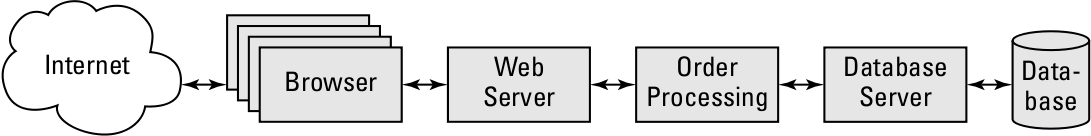
\includegraphics[width=0.85\textwidth]{bilder/soa1.png}}
		\caption[Einfach Software Architektur]{Einfach Software Architektur\protect\footnote}
		\label{soa1}
\end{figure}
\footnotetext{Quelle: \cite{SOA07} S. 18}
Durch den gewöhnlichen Browser können Benutzer auf die Webseite des Webservers zugreifen um dort auf die eigentliche Anwendung des Webshops \textit{Order Processing} zuzugreifen.
Dabei werden durch einen Datenbankserver die Informationen in einer Datenbank gespeichert oder von dort der Webshop-Anwendung zugänglich gemacht.
Welche Funktion die Anwendung \textit{Order Processing} ausführt hängt von den Aufforderungen des Benutzers durch den Browser ab.

Dieser Struktur wird nun ein Service-Orientierte Komponente \textit{Credit Checking} hinzugefügt, siehe Abbildung \ref{soa2}.

\begin{figure}[ht]
	\centering
	   \fbox{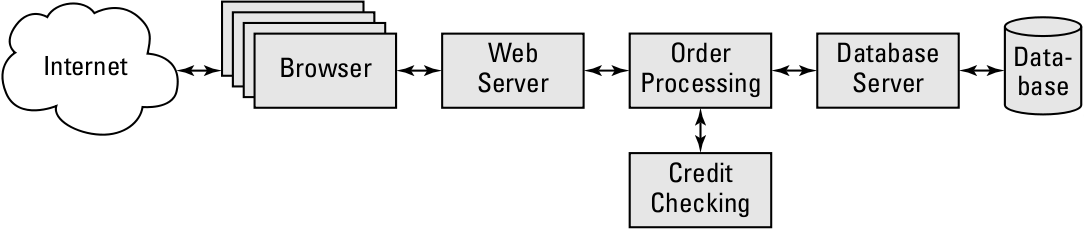
\includegraphics[width=0.85\textwidth]{bilder/soa2.png}}
		\caption[Erweiterte Software Architektur mit Service-Orientierte Komponente]{Erweiterte Software Architektur mit Service-Orientierte Komponente\protect\footnote}
		\label{soa2}
\end{figure}
\footnotetext{Quelle: \cite{SOA07} S. 20}

Dabei hat die eigentliche Anwendung des Webshops keine Kenntniss wie die Komponente \textit{Credit Checking} intern abläuft, sondern übergibt nur die essentiellen Informationen, in diesem Fall die Kreditkartendaten, an die Komponente.
Es ist unrelevant, ob diese Komponenten eine externe Datenbank oder Webseite nach der Kreditwürdigkeit des Benutzers befragen, solange die Komponente auswertbare Informationen (zahlungsfähig ja/nein) an die Webshop Anwendung liefert.
Für die Anwendung \textit{Order Processing} ist die Komponente \textit{Credit Checking} eine sogennante \textbf{black box}.

Die komplexen Berechnungen und Algorithmen zur Bestimmung der Kreditwürdigkeit des Benutzers werden komplett verdeckt, so dass nur die Kreditkarteninformationen der Komponente zu übergeben sind.

Die Komponente \textit{Credit Checking} steht der Webshop Anwendung als \textbf{abstrahierter Dienst bzw. Service} zur Verfügung.